\documentclass[
	% -- opções da classe memoir --
	12pt,				% tamanho da fonte
	oneside,			% para impressão apenas no verso. Oposto a twoside
	a4paper,			% tamanho do papel. 
	english,			% idioma adicional para hifenização
	brazil,				% o último idioma é o principal do documento
	sumario=tradicional
	]{abntex2}
\usepackage[brazil]{babel}
%\usepackage[english]{babel}
\usepackage[utf8]{inputenc}
%\usepackage{subfigure}
\usepackage{algorithm}
\usepackage{array}
\usepackage{multirow}
\usepackage[noend]{algpseudocode}
\usepackage[table]{xcolor}

\usepackage{siunitx}
\usepackage{makecell, booktabs, caption}
\renewcommand\theadfont{\normalsize\bfseries}
\usepackage{amsmath}
\DeclareMathOperator{\Min}{Min}
\DeclareMathOperator{\Max}{Max}

\usepackage[T1]{fontenc}
\usepackage{mwe}    % loads »blindtext« and »graphicx«
\usepackage{subfig}
\usepackage[noend]{algpseudocode}
\graphicspath{ {images/} }

% ---
% PACOTES
% Pacotes fundamentais 
% ---
\usepackage{lmodern}			% Usa a fonte Latin Modern
\usepackage[T1]{fontenc}		% Selecao de codigos de fonte.
\usepackage[utf8]{inputenc}		% Codificacao do documento (conversão automática dos acentos)
\usepackage{indentfirst}		% Indenta o primeiro parágrafo de cada seção.
\usepackage{nomencl} 			% Lista de simbolos
\usepackage{color}				% Controle das cores
\usepackage{graphicx}			% Inclusão de gráficos
\usepackage{microtype} 			% para melhorias de justificação
\usepackage[table]{xcolor}		% permite colocar cor nas tabelas
\usepackage{multirow}			% possibilita mesclar celulas em tabelas
\usepackage{float}
\usepackage{enumitem}			% permite a criação de enumeraçao personalizada
\usepackage{pdfpages}


%----------------------------------------------------------------

\DisemulatePackage{setspace}
\usepackage{setspace}%espaçamento entre linhas 
% ---
% Pacotes adicionais, usados apenas no âmbito do Modelo Canônico do abnteX2
% ---
\usepackage{lipsum}		

\usepackage[brazilian,hyperpageref]{backref}	 % Paginas com as citações na bibl
\usepackage[alf]{abntex2cite}	% Citações padrão ABNT
% ---

%----------------------------------------------------------------

\usepackage{array}
\newcolumntype{C}[1]{>{\centering\let\newline\\\arraybackslash\hspace{0pt}}m{#1}}
\newcolumntype{L}[1]{>{\raggedright\let\newline\\\arraybackslash\hspace{0pt}}m{#1}}


% ---
% Configurações do pacote backref
% Usado sem a opção hyperpageref de backref
\renewcommand{\backrefpagesname}{Citado na(s) página(s):~}
% Texto padrão antes do número das páginas
\renewcommand{\backref}{}
% Define os textos da citação
\renewcommand*{\backrefalt}[4]{
	\ifcase #1 %
		%Nenhuma citação no texto.%
	\or
		%Citado na página #2.%
	\else
		%Citado #1 vezes nas páginas #2.%
	\fi}%
% ---


% ---
% Informações de dados para CAPA e FOLHA DE ROSTO
% ---
\title{Modelo \LaTeX  para contrução de Monografias e Projetos de Pesquisa para as disciplinas de TCC I e II na Ciência da Computação UESPI}
\autor{Ziraldo dos Cocais}
\local{Piripiri-Piauí}
\data{2020}
\preambulo{Trabalho de conclusão de curso de graduação apresentado à
Universidade Estadual do Piauí como requisito parcial para a obtenção de título de Bacharel em Ciência da Computação.

{\vspace{\onelineskip} 
\noindent 
Área de habilitação: Ciência da computação}
}






\orientador{Prof. Dr. Orientador}
\coorientador{Prof. Dr. Coorientador }
\instituicao{Universidade Estadual do Piauí}
\tipotrabalho{monografia}
% ---

% ---
% Configurações de aparência do PDF final

% alterando o aspecto da cor azul
\definecolor{blue}{RGB}{41,5,195}

% informações do PDF
\makeatletter
\hypersetup{
     	%pagebackref=true,
		pdftitle={\@title}, 
		pdfauthor={\@author},
    	pdfsubject={Monogafia escrita com abnTeX2},
	    pdfcreator={LaTeX with abnTeX2},
		pdfkeywords={abnt}{latex}{abntex}{abntex2}{monografia}, 
		colorlinks=true,       		% false: boxed links; true: colored links
    	linkcolor=blue,          	% color of internal links
    	citecolor=blue,        		% color of links to bibliography
    	filecolor=magenta,      		% color of file links
		urlcolor=blue,
		bookmarksdepth=4
}




\makeatother
% --- 

% ---
% compila o indice
% ---objetivos1.2.1
\makeindex
% ---

% ---
% Altera as margens padrões
% ---
\setlrmarginsandblock{3cm}{2cm}{*} %direita e esquerda
\setulmarginsandblock{3cm}{2cm}{*} %cima e baixo
\checkandfixthelayout
% ---

% --- 
% Espaçamentos entre linhas e parágrafos 
% --- 
% O tamanho do parágrafo é dado por:
\setlength{\parindent}{2cm}

% Controle do espaçamento entre um parágrafo e outro:
\setlength{\parskip}{0.2cm}  % tente também \onelineskip

% Espaçamento simples
\onehalfspacing %entre linhas 1.5 padrao

% -----
% Declaracoes de cabecalhos 
% -----
% Cabecalho padrao
\makepagestyle{abntheadings}
\makeevenhead{abntheadings}{\ABNTEXfontereduzida\thepage}{}{\ABNTEXfontereduzida\leftmark}
\makeoddhead{abntheadings}{\ABNTEXfontereduzida}{}{\ABNTEXfontereduzida\thepage}
% Cabecalho do inicio do capitulo
\makepagestyle{abntchapfirst}
\makeoddhead{abntchapfirst}{}{}{\ABNTEXfontereduzida\thepage}
% ----
% ----
% Início do documento
% ----
\begin{document}

\begin{table}[ht]
\centering
\fontsize{10}{16}\selectfont
\begin{tabular}{lcr}
\multirow{3}{*}{\hspace{0cm}
\includegraphics[width=1.25cm]{images/piaui.jpg}} & \textbf{UNIVERSIDADE ESTADUAL DO PIAUÍ - UESPI} & \multirow{3}{*}{
\includegraphics[width=1cm]{images/uespi.jpg}} \\
& \textbf{CAMPUS PROFESSOR ANTÔNIO GIOVANNE ALVES DE SOUSA} & \\
& \textbf{CURSO DE BACHARELADO EM CIÊNCIA DA COMPUTAÇÃO} &
\end{tabular}
\end{table}
\imprimircapa %%Adiciona a compilacao um documento tex

\setcounter{page}{1} %A contagem de pagina começa na folha de rosto sendo a pag.1
\imprimirfolhaderosto

\begin{folhadeaprovacao}
\assinatura{Ziraldo dos Cocais} 
\vspace{1cm}

\begin{center} 
{\ABNTEXchapterfont\large\bfseries\imprimirtitulo}
\end{center}
\imprimirpreambulo 
\vspace{1cm}
\begin{center}
Monografia apresentada em: \_\_/\_\_/\_\_. 
\end{center}

\begin{center}
BANCA EXAMINADORA
\end{center}

\assinatura{Prof. Dr. Orientador \\Universidade Estadual do Piauí - UESPI\\Orientador} 
\assinatura{Prof. Me. Fulano de Tal\\Universidade dele - SIGLA\\Examinador 1}
\assinatura{Prof. Me. Sicrano do Norte \\Instituto dele - IFPI\\Examinador 2} 

\end{folhadeaprovacao} 

\newpage % comentar se for projeto de TCC II
%%%%%%%%%%%%%%%%%%%%%%%%%%%%%%%%% 
% Início da dedicatória - Elemento opcional 
%%%%%%%%%%%%%%%%%%%%%%%%%%%%%%%%%%%%%%%%%%%%%%%%%%%%%%%%%%% 
\begin{dedicatoria} 
\vspace*{\fill} 
\begin{flushright}
\textit{Dedico este trabalho à minha família, em especial meu pai, minha mãe, meu irmão, cacho, gato, papagaio, etc.}
\end{flushright}
\vspace*{\fill} 
\end{dedicatoria}
%%%%%%%%%%%%%%%%%%%%%%%%%%%%%%%%%%%%%%%%%%%%%%%%%% 
% Fim da dedicatória 
%%%%%%%%%%%%%%%%%%%%%%%%%%%%%%%%%%%%%%%%%%%%%%%%%%
\newpage% comentar se for projeto de TCC II
%%%%%%%%%%%%%%%%%%%%%%%%%%%%%%%%%%%%%%%%% 
% Início dos agradecimentos - elemento opcional 
%%%%%%%%%%%%%%%%%%%%%%%%%%%%%%%%%%%%%%%%%%%%%%%%%%%%%%% 

\begin{agradecimentos}[AGRADECIMENTOS]
A Deus primeiramente, por ter me iluminado a cada dia, com coragem, paciência e nunca ter me deixado abalar por nada, apesar da dificuldades;

À minha família, em especial minha mãe Maria dos Remédios de Carvalho Marques, meu pai Francisco das Chagas Fontenele Marques e meu irmão Antonio Lucas de Carvalho Marques, por serem meus espelhos para a vida e por tudo que sempre fizeram, nunca deixando me faltar nada para construção desse sonho, sempre fazendo tudo que esteve ao alcance, com apoio, amor, carinho, dedicação e compreensão, em especial, sem vocês nada disso seria possível;

À Maria do Carmo Silva Carvalho, por todo apoio, conselhos, pela paciência para lidar e enfrentar todas as adversidades ao meu lado, sempre se mostrando uma real e fiel companheira, seja nos momentos de alegria ou aflição;

Aos professores e amigos, Me. Aratã Andrade Saraiva e Me. José Vigno Moura Sousa, por sempre serem presentes e empenhados, que com calma e elegância, sempre souberam repassar todo seu conhecimento de forma bastante profissional e exemplar, além de ter formado um vínculo além de aluno-professor;

Aos meus amigos do Núcleo de Processamento de Dados e de classe, que mesmo de forma direta e indireta contribuíram para o desenvolvimento deste trabalho;

A todo o corpo docente do Curso de Ciência da Computação da Universidade Estadual do Piauí - Campus Piripiri;

Seria difícil citar todos, mas de já, meu muito obrigado a todos que contribuíram diretamente ou não para minha formação.


\end{agradecimentos} 

%%%%%%%%%%%%%%%%%%%%%%%%%%%%%%%%%%%%%%%%%%%%%%%%%%%%%%%%%%% 
%Fim dos agradecimentos - elemento opcional 
%%%%%%%%%%%%%%%%%%%%%%%%%%%%%%%%%%%%%%%%%%%%%%%%%%%%%%%
\newpage% comentar se for projeto de TCC II
%%%%%%%%%%%%%%%%%%%%%%% 
% Início da epígrafe - opcional 
%%%%%%%%%%%%%%%%%%%%%%%%%%%%%%%%%%%%%%%%%%%%%%%%%%%%%%%%%%%%%% 
\begin{epigrafe} 
\vspace*{\fill} 
\begin{flushright} 
\textit{Bem, no mundo real os talentosos ofuscam os barulhentos!\\(Naruto - Masashi Kishimoto)} 
\end{flushright} 
\end{epigrafe} 
%%%%%%%%%%%%%%%%%%%%%%%%%%%%%%%%%%%%%%%%%%%%%%%%%%%%%%%%%%%%%%%%% 
% Fim da epígrafe - opcional 
%%%%%%%%%%%%%%%%%%%%%%%%%%%%%%%%%%%%%%%%%%%%%%%%%%%%%%%%%%%%%%
\newpage% comentar se for projeto de TCC II
%%%%%%%%%%%%%%%%%%%%%%%%%%%%%%%%%%%%%%%%% 
% Início do resumo - obrigatório 
%%%%%%%%%%%%%%%%%%%%%%%%%%%%%%%%%%%%%%%%%%%%%%%%%%%%%%%%%%%%%% 
\begin{resumo}[RESUMO]
		\lipsum[1]

\vspace{\onelineskip} 
\noindent 

\textbf{Palavras-chave}: DICOM. Pseudo-cor. Compressão. Descompressão.
\end{resumo} 
%%%%%%%%%%%%%%%%%%%%%%%%%%%%%%%%%%%%%%%%%%%%%%%%%%%%%%%%%%%%%%%%% 
% Fim do resumo - obrigatório 
%%%%%%%%%%%%%%%%%%%%%%%%%%%%%%%%%%%%%%%%%%%%%%%%%%%%
\newpage
% comentar se for projeto de TCC II
%%%%%%%%%%%%%%%%%%%%%%%%%%%%%%%%%%%%%%%%%%%%%%%%%%%%%%%%%%%%%%%%%
% Início do abstract - obrigatório 
%%%%%%%%%%%%%%%%%%%%%%%%%%%%%%%%%%%%%%%%%%%%%%%%%%%%%%%%%%%%%% 
\begin{resumo}[ABSTRACT] 
\begin{otherlanguage*}{english}

\lipsum[1]

\vspace{\onelineskip} 
\noindent 

\textbf{Keywords}: DICOM. Pseudo Color. Compression. Decompression.
\end{otherlanguage*} 
\end{resumo} 
%%%%%%%%%%%%%%%%%%%%%%%%%%%%%%%%%%%%%%%%%%%%%%%%%%%%%%%%%%%%%%%%% 
% Fim do abstract - obrigatório 
%%%%%%%%%%%%%%%%%%%%%%%%%%%%%%%%%%%%%%%%%%%%%%%%%%%%%%
\newpage

% comentar se for projeto de TCC II

\renewcommand{\listfigurename}{LISTA DE FIGURAS}
\renewcommand{\listtablename}{LISTA DE TABELAS}
\renewcommand{\listadesiglasname}{LISTA DE ABREVIATURAS E SIGLAS}
% ---
% inserir lista de ilustrações
% ---
\pdfbookmark[0]{\listfigurename*}{lof}
\begin{doublespacing}
	\listoffigures*
\end{doublespacing}
\cleardoublepage
% ---

% ---
% inserir lista de tabelas
% ---
\pdfbookmark[0]{\listtablename*}{lot}
\begin{doublespacing}
\listoftables*
\end{doublespacing}
\cleardoublepage
% ---

% ---
% inserir lista de abreviaturas e siglas
% ---
\begin{doublespacing}
\begin{siglas}
\item [ARP] \textit{Aprendizado por Reforço Profundo}
\item [AR] \textit{Aprendizagem por reforço}
\item [IA] \textit{Inteligência Artificial}
\item [ARPMG] \textit{Aprendizado por reforço profundo  Multi-Agente}
\item [MDP] \textit{Processo de Decisão Markoviano}
\item [MLP] \textit{Multilayer perceptron}
\end{siglas}
\end{doublespacing}
%% ---
\pdfbookmark[0]{\contentsname}{toc}
\tableofcontents*
\cleardoublepage
%% ---

%%%%%%%%%%%%%%%%%%%%%%%%%%%%%%%%%%%%%%%%%%%%%%%%%%%%%%%%%%%%%%%%% 
% Inicio dos Capitulos
%%%%%%%%%%%%%%%%%%%%%%%%%%%%%%%%%%%%%%%%%%%%%%%%%%%%%%
% Introducao

\chapter{INTRODUÇÃO}

Aqui você pode apresentar o capítulo de introdução do seu trabalho, além de algumas definições de conceitos utilizados no decorrer do seu  texto. Em seguida você vai ler 3 parágrafos de Lorem ipsum para encher linguíça.
 
\lipsum[3-5]


\section{Justificativa}

Esta seção deve apresentar a justificafiva para escolha do tema, a importância (e/ou relevância) de trabalhar o tema escolhido.


\section{Objetivos}

Os objetivos do seu trabalho vem em seguida e são divididos em duas partes:  Geral e Específicos.

\subsection{Objetivo geral}
O objetivo principal deste trabalho é mostrar para os alunos como escrever uma monografia utilizado o modelo \LaTeX.

\subsection{Objetivos específicos}

\begin{itemize}
 
	\item Escrever texto explicativo de cada parte do modelo;
	\item Disponibilizar o modelo \LaTeX em um repositório \texttt{Git}.
\end{itemize}


\section{Fora do Escopo}
Nesta seção você pode enumerar as coisas que estam fora do escopo do seu trabalho de conclusão.
\begin{description}
	\item[Ponto 1] Não é do escopo deste trabalho mostrar como você escolhe o tema do \emph{seu}  trabalho de conclusão de curso;
	\item[Ponto 2 ]  Não é do escopo deste trabalho mostrar como gerir o seu tempo para concluir o \emph{seu}  trabalho de conclusão de curso; 
	\item[Ponto 3] Não é do escopo deste trabalho escolher o orientador para o \emph{seu}  trabalho de conclusão de curso; 
	\item[Ponto 4] Não é do escopo deste trabalho escrever o \emph{seu}  trabalho de conclusão de curso.
\end{description}

\section{Organização do documento}

O restante deste documento é organizado como segue. O Capítulo \ref{cap:referencial} apresenta o referêncial teórico. O Capítulo \ref{cap:metodo} apresenta a metodologia utilizada. O Capítulo \ref{cap:cronograma} o cronograma para o seu Trabalho de Conclusão de Curso II, caso esteja fazendo o seu projeto de TCC. apresenta os resultados obtidos e por fim o Capítulo \ref{cap:conclusao} apresenta conclusões e trabalhos futuros.
\newpage
\chapter{REFERENCIAL TEÓRICO}\label{cap:referencial}

Este capítulo deve apresentar o referencial teórico para o seu TCC. Isto pode incluir:  \textit{(i)} uma breve apresentação da subárea em que seu trabalho está incluído;  \textit{(ii)} apresentação de rabalhos relacionados publicados em conferências nacionais, internacionais e periódicos;  \textit{(iii) produtos de software relacionados ao que você desenvolveu/melhorou}. Em seguida você vai ler 3 parágrafos de Lorem ipsum para encher linguíça.

\lipsum[3-5]




\newpage
\chapter{METODOLOGIA}\label{cap:metodo}
Neste capítulo é apresentado a fundamentação teórica, onde é descrito detalhadamente o método utilizado no desenvolvimento do  trabalho. Em seguida você vai ler 3 parágrafos de Lorem ipsum para encher linguíça.

\lipsum[3-5]



\section{Inserção de Imagens} \label{sec:imagens}
A figura \ref{fig:metodo} apresenta um exemplo de como adicionar uma imagem ao seu trabalho. Em seguida você vai ler 2 parágrafos de Lorem ipsum para encher linguíça.

\lipsum[2-4]


\begin{figure}[H]
\centering
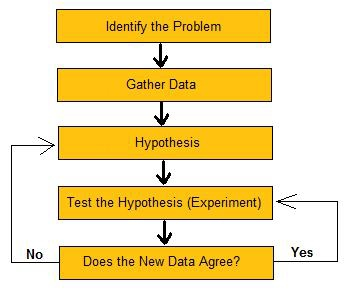
\includegraphics[width=11cm, height =9cm]{images/The_Scientific_Method.jpg}
\caption{Exemplo de metodologia em inglês.}
\legend{Fonte: Retirado da Wikimedia Commons.}
\label{fig:metodo}
\end{figure}

\subsection{Como fazer uma subseção}
Em seguida você vai ler 2 parágrafos de Lorem ipsum para encher linguíça.

\lipsum[2-4]
\subsection{Outra subseção}
Em seguida você vai ler 2 parágrafos de Lorem ipsum para encher linguíça.

\lipsum[2-4]
\section{Passo 2: Referências às seções do documento}\label{sec:refs}

Não adicione uma Seção \ref{sec:imagens} se você não tem uma Seção \ref{sec:refs} em seguida.  Em seguida você vai ler 2 parágrafos de Lorem ipsum para encher linguíça.

\lipsum[2-4]



\newpage
\chapter{RESULTADOS}\label{cap:resultados}


Neste capítulo você apresenta os resultados obtidos após a execução de todos os passos descritos na metodologia. É possível apresntar aqui também uma discussão crítica sobre os resultados otidos.  Uma outra opção é criar um capítulo somente a discussão dos resultados e lições aprendidas.

Este capítulo só existe se você tiver concluindo o TCC II. Caso contrário, você pode enumerar o \textbf{RESULTADOS ESPERADOS}.



\newpage
\chapter{CRONOGRAMA}\label{cap:cronograma}

Neste capítulo você deve descrever o seu cronograma de conclusão se você estiver escrevendo o seu projeto. Naturalmente, caso esteja escrevendo o documento para a apresentação final este capítulo não é necessário.


A Tabela \ref{tab:cronograma} apresenta o cronograma. Mas você deve descrever brevemente cada uma das atividades nele indicadas: 
\begin{description}
	\item[Tarefa 1:] descrição da tarefa 1;
	\item[Tarefa 2:] descrição da tarefa 2;
	\item[Tarefa 3:] descrição da tarefa 3;
	\item[\ldots:] descrição da tarefa \ldots;
	\item[Mais uma Tarefa:] descrição de mais uma tarefa ;
	\item[\ldots:] descrição da tarefa \ldots;
	\item[Tarefa final:] descrição da tarefa final;
\end{description}


% Please add the following required packages to your document preamble:
% \usepackage{multirow}
\begin{table}[h]
	\caption{Cronograma de atividades do Trabalho de Conclusão de Curso II.}
\centering
\fontsize{5}{11}\selectfont
\begin{tabular}{|l|c|c|c|c|c|c|c|c|c|c|c|c|c|}
\hline
\multicolumn{1}{|c|}{\multirow{3}{*}{\textbf{ATIVIDADES}}} & \multicolumn{12}{c|}{\textbf{MESES}}                                                                          \\ \cline{2-13} 
\multicolumn{1}{|c|}{}                                     & \multicolumn{12}{c|}{\textbf{2021}}                                                                        \\ \cline{2-13} 
\multicolumn{1}{|c|}{}     & \multicolumn{1}{l|}{\textbf{Jul}} & \multicolumn{1}{l|}{\textbf{Ago}} & \multicolumn{1}{l|}{\textbf{Set}} & \multicolumn{1}{l|}{\textbf{Out}} & \multicolumn{1}{l|}{\textbf{Nov}} & \multicolumn{1}{l|}{\textbf{Dez}} & \multicolumn{1}{l|}{\textbf{Jan}} & \multicolumn{1}{l|}{\textbf{Fev}} & \multicolumn{1}{l|}{\textbf{Mar}} & \multicolumn{1}{l|}{\textbf{Abr}} & \multicolumn{1}{l|}{\textbf{Mai}} & \multicolumn{1}{l|}{\textbf{Jun}}  \\ \hline
Tarefa 1 & x& x& x& x& x& x& x& x& x& x& x& x \\ \hline
Tarefa 2& & & & & & & x & & & & & \\ \hline
Tarefa 3&x &x &x &x &x  &x  &x  &x  &x  &x  & x &  \\ \hline
\ldots &x &x &x &x &x  &x  &  &  &  &  &  &  \\ \hline
Mais uma tarefa &x &x &x &x &x &x &x &x &x &x &x &x  \\ \hline
\ldots&x &x &x &x &x  &x  &x  &x  &x  &x  &x  &x  \\ \hline
Tarefa final & & & & & & & & & & & &\\ \hline
\end{tabular}
\label{tab:cronograma}
\end{table}

 % comentar se for TCC II
\newpage
\chapter{CONCLUSÃO}\label{cap:conclusao}


Neste capítulo você apresenta as conclusões do seu trabalho. É comum, também aprsesentar direções para trablahos futuros que possam vir a dar continuidade ao trabalho que você executou.

Este capítulo só existe se você tiver concluindo o TCC II. 


% comentar se for projeto de TCC II



%\input{sumario.tex}
%Abaixo o inicio da paginacao e do trabalho textual
\pagestyle{abntheadings} % insere a paginacao nas paginas que nao sao capitulos
\aliaspagestyle{chapter}{abntchapfirst}% insere a paginacao nos capitulos


%\newpage
\chapter{CONCLUSÃO}\label{cap:conclusao}


Neste capítulo você apresenta as conclusões do seu trabalho. É comum, também aprsesentar direções para trablahos futuros que possam vir a dar continuidade ao trabalho que você executou.

Este capítulo só existe se você tiver concluindo o TCC II. 



\newpage
%Abaixo conteudo extra textual

% ----------------------------------------------------------
% Apêndices
% ----------------------------------------------------------
% ---
% Inicia os apêndices
% ---

	% ---
	%\begin{apendicesenv}
		
		% Imprime uma página indicando o início dos apêndices
		%\partapendices
		
		% ----------------------------------------------------------
		%\input{apendice.tex}
		
	%\end{apendicesenv}

\newpage
%\input{cap/outracitacao.tex}
\bibliographystyle{abntex2-alf}
%\bibliography{references}


%\begin{apendicesenv}
% Imprime uma página indicando o início dos apêndices
%\partapendices


%\input{cap/apendiceC.tex}


%\end{apendicesenv}
% ----------------------------------------------------------
% Anexos
% ----------------------------------------------------------
% ---
% Inicia os anexos
% ---
%\begin{anexosenv}
% Imprime uma página indicando o início dos anexos
%\partanexos

\newpage
%\chapter{Resultados parciais}

%artigo-scalable-task.pdf
%\includepdf[pages=-]{artigo-scalable-task}

\renewcommand\bibname{REFERÊNCIAS}
\bibliography{references}
%\end{anexosenv}
\end{document}


